\documentclass[12pt, xcolor=dvipsnames]{scrartcl}

% include packages
% sonderzeichen encoding
% sonderzeichen encoding
\usepackage[utf8]{inputenc}
\usepackage[T1]{fontenc}
\usepackage[ngerman]{babel}

% xcolor package
\usepackage[dvipsnames,table]{xcolor}

% tables package & alternierende rowcolors in Tabellen
% alternating rowcolors in tables
\usepackage{longtable}
\rowcolors{2}{gray!15}{white}

% bilder
% bilder
\usepackage{graphicx}

% pdf includes
% pdf includes
\usepackage{pdfpages}

% toc als links rendern
% toc als links rendern
\usepackage[hidelinks]{hyperref}

% listings (source code)
%listing (source code)
\usepackage{listings}
\lstdefinelanguage{JavaScript}{
  keywords={typeof, new, true, false, catch, function, return, null, catch, switch, var, if, in, while, do, else, case, break},
  keywordstyle=\color{blue}\bfseries,
  ndkeywords={class, export, boolean, throw, implements, import, this},
  ndkeywordstyle=\color{darkgray}\bfseries,
  identifierstyle=\color{black},
  sensitive=false,
  comment=[l]{//},
  morecomment=[s]{/*}{*/},
  commentstyle=\color{purple}\ttfamily,
  stringstyle=\color{red}\ttfamily,
  morestring=[b]',
  morestring=[b]"
}

\lstset{
   language=JavaScript,
   backgroundcolor=\color{lightgray!50},
   extendedchars=true,
   basicstyle=\footnotesize\ttfamily,
   showstringspaces=false,
   showspaces=false,
   numbers=left,
   numberstyle=\footnotesize,
   numbersep=9pt,
   tabsize=2,
   breaklines=true,
   showtabs=false,
   captionpos=b
}

% show lof and lot in toc
% show lof and lot in toc
\usepackage[nottoc]{tocbibind}

% appendix
% appendix package
\usepackage[toc,page]{appendix}

% deutscher appendix name
\addto\captionsngerman{\let\appendixtocname\appendixname%
\let\appendixpagename\appendixname}

% nomencl (Abkuerzungsverzeichnis)
\usepackage[intoc]{nomencl}
\let\abbrev\nomenclature
\renewcommand{\nomname}{Abk\"urzungsverzeichnis}
\setlength{\nomlabelwidth}{7em}
\renewcommand{\nomlabel}[1]{#1 \dotfill}
\setlength{\nomitemsep}{-\parsep}

% einr�ckung for nomenclature
\usepackage{xstring}
\usepackage{xpatch}
\patchcmd{\thenomenclature}
  {\leftmargin\labelwidth}
  {\leftmargin\labelwidth\itemindent 1em }
  {}{}

\newcommand{\nomenclheader}[1]{%
  \item[\hspace*{-\itemindent}\normalfont\bfseries#1]}


\makenomenclature 

% ben�tigt f�r float angaben an tables, z.B. \begin{tyble}[H]
\usepackage{float}


% ben�tigt f�r \being{savenotes}, um fu�noten in tabellen zu verwenden
\usepackage{footnote}

% eurozeichen
\usepackage{eurosym}
\usepackage{textcomp}
\usepackage{amstext} % for \text
\DeclareRobustCommand{\officialeuro}{%
  \ifmmode\expandafter\text\fi
  {\fontencoding{U}\fontfamily{eurosym}\selectfont e}}


% used for linebreaks in table cells
\usepackage{pbox}

% amsmath, f�r aligned environment
\usepackage{amsmath}

% images in header & footer
% images in header & footer
% images in header & footer
\usepackage{fancyhdr}
\pagestyle{fancy}
\rhead{
\includegraphics[width=2cm]{images/gns}}

\newcommand{\timeAnalyse}{9h}
\newcommand{\timeAnalyseDiff}{+ 2h}

\newcommand{\timeEntwurf}{17h}
\newcommand{\timeEntwurfDiff}{- 1h}

\newcommand{\timeImplementierung}{31h}
\newcommand{\timeImplementierungDiff}{+ 5h}

\newcommand{\timeAbnahme}{1h}
\newcommand{\timeAbnahmeDiff}{}

\newcommand{\timeEinfuehrung}{1h}
\newcommand{\timeEinfuehrungDiff}{- 1h}

\newcommand{\timeDokumentation}{11h}
\newcommand{\timeDokumentationDiff}{- 1h}


\begin{document}


\newcommand{\Projekt}{Erstellung einer Webanwendung
		zur Verbesserung des Workflows des Erstellens von Benutzerhandbüchern}

\thispagestyle{empty}

\begin{center}
	\huge \bfseries
	Projektberich: \Projekt \\[4cm]

	\Large	\mdseries

	\textbf{Auszubildender} \\
	Oliver Herrmann \\
	Geb.: 23.09.1992 \\
	GNS mbH \\
	Tel.: +49 201 109 - 1523 \\
	Email: \href{mailto:oliver.herrmann@gns.de}{oliver.herrmann@gns.de}  \\
	Ausbildungsberuf: Fachinformatiker Anwendungsentwicklung \\[2cm]

	\textbf{Ausbildungsbetrieb} \\
	GNS mbH \\
	Frohnhauser Str. 67 \\
	45127 Essen \\[3cm]

	\today, Essen
\end{center}



\clearpage

% Letzter parameter ist numbering width in ToC
\makeatletter
  \renewcommand\l@subsection{\@dottedtocline{2}{1.5em}{2.8em}}
\makeatother
\addcontentsline{toc}{section}{Inhaltsverzeichnis}
\tableofcontents

% \clearpage

\listoffigures
% \clearpage

\listoftables
% \clearpage

\lstlistoflistings
% \clearpage

\abbrev{KIS}{Abteilung der GNS für Softwareentwicklung}
\abbrev{GNS}{Gesellschaft für Nuklear-Service mbH}	
\abbrev{Hosting}{Bereitstellen einer Web-Anwendung auf einem Web-Server}	
\abbrev{CVS}{Concurrent Version System}	
\abbrev{REST}{Representational State Transfer}	
\abbrev{JSON}{JavaScript Object Notation}
\abbrev{HTTP}{Hypertext Transfer Protocol}
\abbrev{HTML}{Hypertext Markup Language}
\abbrev{CSS}{Cascading Style Sheets}
\abbrev{URL}{Uniform Resource Locator}
\abbrev{JEE}{Java Platform, Enterprise Edition}
\abbrev{API}{Application Programming Interface}
\abbrev{GUI}{Graphical User Interface}
\printnomenclature		
\clearpage



\section{Einleitung}

\subsection{Projektumfeld}
\label{sec:projektumfeld}

Die GNS (Gesellschaft für Nuklear-Service) mbH ist ein mittelständisches Unternehmen, das 1977 gegründet wurde und aktuell etwa 550 Mitarbeiter beschäftigt. Die Firmenzentrale befindet sich in Essen. Die GNS betreibt des Weiteren Standorte in Duisburg, Mülheim an der Ruhr und Karlsruhe. Das Hauptgeschäftsfeld der GNS ist die Entwicklung, sowie der Vertrieb von Behältern zur Lagerung und zum Transport von radioaktivem Material, als auch die Beladung solcher Behältnisse.


Ebenfalls zum Geschäftsbereich der GNS zugehörig ist der Ver- und Betrieb von Softwarelösungen. Hier ist beispielhaft das AVK(Abfallfluss- Verfolgungs- und Produktkontroll-System) zu nennen, welches 1991 entwickelt wurde und heute in allen deutschen Kernkraftwerken verwendet wird.  Daneben werden von der GNS eine Vielzahl von stark spezialisierten Softwarelösungen betrieben, wovon viele als digitale Dienstleistung für Kunden (z.B. Kernkraftwerke und Zwischenlager) bereitgestellt werden. \\

Auftraggeber des Projekts ''\Projekt'' ist die GNS, in Person Friedrich Bauriedel, Leiter der Abteilung KIS.


\subsection{Projektziel}

Ziel des Projekts ist, den regelmäßig anfallenden Arbeitsschritt ''Erstellen eines Benutzerhandbuchs aus einem Wiki'' für die Mitarbeiter der GNS zu vereinfachen und zu beschleunigen. Ebenfalls soll der Workflow normiert und zentralisiert werden, sodass der Aufwand für vorlaufende Arbeiten minimiert wird.

\subsection{Projektbegründung}
\label{sec:projektbegründung}

Wie in Abschnitt \ref{sec:projektumfeld} erwähnt, betreibt die GNS eine Vielzahl an hoch spezialisierten Softwarelösungen für diverse Kunden. Aufgrund der Komplexität vieler dieser Anwendungen ist es nötig, den Benutzern ein Handbuch zur Verfügung zu stellen.
Zu diesem Zweck betreibt die GNS betriebsinterne Wikis, in denen Inhalte bezüglich der korrekten Bedienung einer Anwendung von Mitarbeitern der GNS gepflegt werden. \\

2012 wurde von der GNS der sogenannte ''WikiConverter'' entwickelt. Dies ist ein Tool, welches die Inhalte eines MediaWikis extrahiert und diese in ein PDF- bzw. HTML-Dokument konvertiert.
Ziel der Entwicklung war es, die mithilfe des WikiConverters erzeugten Dateien als interaktive Hilfe in die jeweiligen Anwendungen einzubetten bzw. als Benutzerhandbuch den Kunden bereitstellen zu können.

Allerdings wurde bei der Entwicklung des WikiConverters wenig Wert auf eine intuitive Benutzerführung gelegt, was dazu führte, dass die Bedienung von diesem äußerst komplex ist. \\

Durch die in den letzten Jahren gesteigerte Anzahl der von der GNS betriebenen Softwarelösungen, sowie die stetige Verkürzung der Release-Intervalle dieser, ist der Arbeitsschritt ''Erstellen von Benutzerhandbüchern'' immer mehr in den Vordergrund gerückt, was schließlich dazu führte, dass eine Überarbeitung von diesem unumgänglich wurde. \\

Zu diesem Zweck wurde von der Abteilung KIS Mitte 2015 das Projekt ''\Projekt'' initiiert, welches zum Ziel hat, die Erstellung von Benutzerhandbüchern zu vereinfachen und zu zentralisieren.

Im Rahmen des Projekts wird eine Web-Anwendung entwickelt, welche die Kernfunktionalität des WikiConverters ummantelt und eine einheitliche, graphische Benutzerschnittstelle zu dieser anbietet. So wird die Komplexität des WikiConverters vor den Benutzern verborgen, um diesen eine einfachere und intuitivere Benutzung zu ermöglichen. \\

Als messbares Ziel des Projekts ist eine Reduzierung der durchschnittlichen Arbeitszeit für den Workflow ''Erstellen eines Benutzerhandbuchs'' um mindestens 25\% veranschlagt.


\subsection{Projektschnittstellen}

Die technischen und sozialen Schnittstellen des Projekts sind ausschließlich betriebsinterner Natur. \\
Technisch betrachtet greift das Projekt die bestehende Anwendung ''WikiConverter'' auf und adaptiert deren Kernfunktionalität. \\
Aus projektspezifischer Sicht sind die Schnittstellen rein intern, da sowohl Auftraggeber als auch Endnutzer der Anwendung Mitarbeiter bzw. Abteilungen der GNS sind. \\
Die projektabschließende Abnahme erfolgt gegenüber dem Auftraggeber, hier die Abteilung KIS der GNS.


\subsection{Projektabgrenzung}
\label{sec:projektabgrenzung}

Ausdrücklich nicht Teil des Projekts ist das Hosting der im Rahmen des Projekts entwickelten Anwendung sowie alle in Verbindung mit dem Hosting stehenden administrativen Maßnahmen. Diese werden von nicht direkt am Projekt beteiligten Mitarbeitern der GNS durchgeführt.


\section{Projektplanung}

\subsection{Projektphasen} \label{sec:projektphasen}

	\begin{table}[H]
	\centering
	\begin{tabular}{lr}

		\rowcolor{white!15}				
		\textbf{Projekphase} & \textbf{Geplante Zeit} \\\hline
		
	    Anforderungsanalyse & 7h \\	   	   
	    Projektplanung & 4h \\	   			
	    Software-Architektur & 14h \\	 				
	    Implementierung & 26h \\	   				
	    Projektabschluss & 3h \\	   				
	    Sonstiges & 16h \\\hline
	  		
		\rowcolor{white!15}				
		\textbf{Gesamt} & \textbf{70h}				
			    
	\end{tabular}
	\caption{Projektphasen}
	\label{tab:projektphasen}
	\end{table}
	
	Eine detaillierte Übersicht der einzelnen Phasen findet sich im Anhang \ref{app:projektphasen_detail} auf Seite \pageref{app:projektphasen_detail}
	

\subsection{Abweichung vom Projektantrag}

Abweichend vom Projektantrag werden das Pflichten- sowie das Lastenheft nur in Auszügen im Projektbericht aufgeführt. Dies ist dem Umfang des vorliegenden Projektberichts geschuldet.

\subsection{Resourcenplanung}

Im Folgenden werden alle für die Durchführung des Projekts benötigten Resourcen aufgelistet. Diese werden durch den Auftraggeber, hier die GNS, bereitgestellt.

\begin{savenotes}
\begin{table}[H]
	\centering
	\begin{tabular}{ll}

		\rowcolor{white!15}				
		\textbf{Art der Resource} & \textbf{Beschreibung} \\\hline		
		
		\rowcolor{MidnightBlue!15}				
		\textbf{Sachliche Ressourcen} & \\
		Projektbüro & \\
		Computer & \\
		\hspace{1.5em} IDE & Eclipse for JEE Developers\footnote{\url{http://www.eclipse.org/downloads/packages/eclipse-ide-java-ee-developers/mars1}, abgerufen am 27.10.2015} \\
		Demilitarisierte Zone & zu Testzwecken \\
		
		\rowcolor{MidnightBlue!15}			
		\textbf{Personelle Ressourcen} & \\
		Projektleiter & Oliver Herrmann \\
		Projektmitarbeiter & Oliver Herrmann \\
	
			    
	\end{tabular}
	\caption{Ressourcen}
	\label{tab:ressourcen}
\end{table}
\end{savenotes}

\subsection{Entwicklungsprozess}

Grundlage für den Entwicklungsprozess bildet das iterative
Wasserfallmodell\footnote{\url{http://www.pi.informatik.tu-darmstadt.de/fileadmin/user_upload/Group_PI/LV__SE_RE/R_01_Wasserfallmodell__Ausarbeitung__Schwaiger.pdf} abgerufen am 05.10.2015}.
Dies wurde gewählt, da es gut mit Projekten geringen bis mittleren Umfangs harmoniert. Andere Modelle wie z.B. Scrum oder Extreme-Programming wurden nicht in Erwägung gezogen, da sie die Projektarbeit im Team voraussetzen.

\section{Analysephase}

\subsection{Ist-Analyse}

Der jetzige Stand bezüglich des Workflows ''Erstellen eines Benutzerhandbuchs'' sieht vor, dass der ausführende Mitarbeiter den WikiConverter aus dem internen CVS auscheckt, im Quellcode Angaben zu dem zu konvertierenden Wiki (URL, Hauptseite) ergänzt und den Quellcode anschließend kompiliert und ausführt. Das Ergebnis der Ausführung sind die generierten PDF- und HTML-Dateien.

Das Projekt ''\Projekt'' definiert den überarbeiteten Workflow wie folgt:

\begin{itemize}
	\item Der Benutzer loggt sich online in der Anwendung ein.
	\item Der Benutzer wählt ein existierendes Wiki aus oder pflegt ein neues ein. (Nötige Angaben sind URL und Hauptseite des Wikis)
	\item Der Benutzer kann über die graphische Oberfläche das Konvertieren starten.
	\item Nach erfolgreicher Konvertierung kann der Benutzer die generierten Dateien herunterladen.
\end{itemize}

Außerdem werden aus Konvertierungsvorgängen erstellte Dateien dauerhaft gespeichert. Diese können ebenfalls vom Benutzer heruntergeladen werden, falls eine neue Konvertierung nicht benötigt wird.

\subsection{Wirtschaftlichkeitsanalyse}
\label{sec:wirtschaftlichkeitsanalyse}

Im Folgenden wird die Wirtschaftlichkeit des Projekts betrachtet. Da das Projekt keinen direkten Gewinn erwirtschaftet, sondern der monetäre Vorteil durch die Erleichterung der Arbeit der betroffenen Mitarbeiter erzielt wird, wird zuerst der Nutzen des Projekts messbar festgehalten. Dieser wird dann den Kosten des Projekts gegenübergestellt, um eine qualifizierte Aussage über die Wirtschaftlichkeit des Projekts zu machen.

Grundlage der Analyse sind folgende Stundensätze\footnote{Beruhend auf Tarifverträgen bzw. betriebsinternen Angaben}:

\begin{table}[H]
	\centering
	\begin{tabular}{lr}

		\rowcolor{white!15}				
		\textbf{Art der Beschäftigung} & \textbf{Stundensatz} \\\hline		
		
		Fachinformatiker & 20 \euro \\
		Auszubildender & 6 \euro \\
		Gemeinkosten & 10 \euro \\
			    
	\end{tabular}
	\caption{Stundensätze}
	\label{tab:stundensätze}
\end{table}

Hieraus ergibt sich ein \textit{effektiver} Stundensatz von 30 \euro{} für die Arbeit eines Fachinformatikers, bzw. 16 \euro{} für die Arbeit eines Auszubildenden (hier Projektmitarbeiter).


\subsubsection{Nutzen des Projekts}
\label{sec:nutzen_des_projekts}

Der Nutzen des Projekts manifestiert sich primär darin, dass der regelmäßig auftretende Workflow ''Erstellen eines Benutzerhandbuchs'' beschleunigt wird.
Da die exakte Bestimmung der durchschnittlich für diesen Workflow anfallenden Zeit von vielen, auch personellen, Faktoren abhängt, wird er für die Zwecke der Wirtschaftlichkeitsanalyse konservativ abgeschätzt. Diese Schätzung wird fortan als Grundlage für weitere Berechnungen herangezogen, um so ein Worst-Case Ergebnis ausdrücken zu können.
Der aktuelle durchschnittliche zeitliche Aufwand für den Workflow ergibt sich aus
\begin{itemize}
	\item Einarbeitung in den Workflow und den WikiConverter im Allgemeinen
	\item Auschecken der Quellen
	\item Anpassungen am Quellcode
	\item Kompilieren der Quellen
	\item Ausführen der Anwendung
	\item Sichern der Ergebnisse
\end{itemize}
und beträgt schätzungsweise \textbf{15 Minuten}. \\

Der neue, vom Projekt angestrebte Workflow setzt sich dagegen wie folgt zusammen: \\

Alternative 1
\begin{itemize}
	\item Login
	\item Konvertierung anstoßen
	\item Herunterladen der Ergebnisse
\end{itemize}
Geschätzte Dauer: \textbf{5 Minuten}. \\

Alternative 2
\begin{itemize}
	\item Login
	\item Auswählen eines bereits existierenden Ergebnisses
	\item Herunterladen der Ergebnisse
\end{itemize}
Geschätzte Dauer: \textbf{2 Minuten}. \\


Hier ist anzumerken, dass durch die zentrale Speicherung der konvertierten Ergebnisse dem Nutzer ermöglicht wird, den zeitintensiven Schritt der Konvertierung auszulassen, wenn ein adäquates Ergebnis bereits existiert. Dies ist z.B dann der Fall, wenn die Konvertierung kürzlich durch einen dritten Mitarbeiter vorgenommen wurde und seitdem keine relevanten Änderungen am zu Grunde liegenden Wiki auftraten.

Konservativ betrachtet wird davon ausgegangen, dass in 80\% der Fälle Alternative 1 und in den übrigen 20\% Alternative 2 eintreten wird.
\begin{equation} \label{eq:t_workflow_durchschn}
	T_\emptyset = 0.8 * 5m + 0.2* 2m = 4.4m
\end{equation}

Aus Formel \ref{eq:t_workflow_durchschn} ergibt sich eine durchschnittliche Dauer des Workflows von \textbf{4,4 Minuten}.


\begin{equation} \label{eq:t_workflow_delta_abs}
	T_{\Delta abs} = 15m-4,4m = 10,6m
\end{equation}

\begin{equation} \label{eq:t_workflow_delta_rel}
	T_{\Delta rel} = \frac{T_{\Delta abs}}{15m} = 71\%
\end{equation}

Dies entspricht nach Formel \ref{eq:t_workflow_delta_rel} einer Einsparung von \textbf{71 \%} und verspricht ein Einhalten des in Kapitel \ref{sec:projektbegründung} ausgesprochenen Ziels, die durchschnittliche Arbeitszeit des Workflows um mindestens mindestens 25\% zu reduzieren. \\

\begin{equation} \label{eq:t_workflow_delta_jahr}
\begin{split}
	T_{\Delta jahr}	&= T_{\Delta abs} * N_{Workflow/Monat} * N_{Monat/Jahr} \\
					& = T_{\Delta abs} * 10 * 12 = 1272m \\
					& = 21,2h
\end{split}
\end{equation}

\begin{equation} \label{eq:k_workflow_jahr}
\begin{split}
	E_{jahr}	&= T_{\Delta jahr} *  Stundensatz_{Mitarbeiter} \\
				& = T_{\Delta jahr} *  \frac{30 \euro}{h} \\
				& = 636 \euro
\end{split}
\end{equation}

Unter der Annahme, dass der Workflow durchschnittlich zehnmal pro Monat von einem Fachangestellten durchgeführt wird, ergibt sich daraus eine Zeitersparnis von 21,2 Stunden pro Jahr, was nach Formel \ref{eq:k_workflow_jahr} einer jährlichen monetären Ersparnis von \textbf{636 \euro{}} entspricht.


\subsubsection{Kosten des Projekts}
\label{sec:kosten_des_projekts}

Die Kosten des Projekts werden allein durch die Kosten der Entwicklung bestimmt. Es werden keine nicht bereits vorhandenen Ressourcen für das Projekt verwendet.
\begin{equation} \label{eq:4}
\begin{split}
	K_{ges}	&= T_{Projekt} * Stundensatz_{Projekt-Mitarbeiter} \\
			& = 70h * \frac{16 \euro}{h} \\
			& = 1120 \euro
\end{split}
\end{equation}
Bei einem kalkulierten Projektumfang von 70 Stunden ergibt sich aus Formel \ref{eq:4} ein Kostenumfang von \textbf{1120 \euro{}}, unter der Voraussetzung, dass als Projektmitarbeiter ausschließlich ein Auszubildender eingesetzt wird. \\


Eine detaillierte, nach Phasen unterteilte Übersicht der Kosten findet sich im Anhang \ref{app:kosten} auf Seite \pageref{app:kosten}

\subsubsection{Amortisationsdauer}

\begin{equation} \label{eq:amort}
	T_{amortisation} = \frac{K_{ges}}{E_{jahr} / a} = \frac{1120 \euro}{636 \euro / a} = 1,76a
\end{equation}

Zieht man die Ergebnisse aus Kapitel \ref{sec:nutzen_des_projekts} und \ref{sec:kosten_des_projekts} heran und betrachtet diese relativ zueinander, wie in Formel \ref{eq:amort} geschehen, lässt sich feststellen, dass sich das Projekt nach etwa 1,8 Jahren amortisiert hat.



\subsection{Risikoanalyse}

Im Folgenden wird eine Risikoanalyse und -bewertung durchgeführt.
Eine detaillierte Übersicht der Risikobewertung findet sich im Anhang \ref{app:risikoanalyse} auf Seite \pageref{app:risikoanalyse}.

Zusammenfassend lässt sich das Ergebnis der Risikoanalyse in drei Teilbereiche gruppieren.

\paragraph{Gruppe 1}
Unvermeidbare Risiken \\
Hierzu zählen z.B. krankheitsbedingte personelle Ausfälle. Diese stellen ein unvermeidbares Risiko dar. Eine Strategie zur Vermeidung ist hier nicht vorgesehen.\\

\paragraph{Gruppe 2}
Bedingt vermeidbare Risiken \\
Hierzu zählen vor allem Risiken aus Fehlern der Planung. Diese Risiken sind bedingt vermeidbar. Dem Auftreten solcher Risiken wird insbesondere durch die im  Qualitätssicherungskonzept vorgesehenen Zwischenstandsanalysen entgegengewirkt.

\paragraph{Gruppe 3}
Leicht vermeidbare Risiken \\
Dies sind in erster Linie Risiken, die in der Entwicklung auftreten können. Das Eintreten dieser Risiken wird primär durch die Erfahrung und intensive fachliche Vorbereitung des Projektmitarbeiters vermieden. Des Weiteren hilft das im Qualitätssicherungskonzept beinhaltete Testkonzept hier für eine frühzeitige Erkennung von Konsequenzen dieser Risikogruppe. \\

Die möglichen Konsequenzen lassen sich wiederum in zwei Bereiche gruppieren.

\paragraph{Gruppe A} Zeitliche Konsequenzen \\
Dies sind Risikofolgen, welche in erster Linie eine Ausdehnung des Projektzeitraums bzw. eine Verzögerung des Projektabschlusses mit sich ziehen. Da das Projekt allerdings für rein betriebsinterne Zwecke konzipiert ist und keinen direkten Gewinn erwirtschaftet, beschränken sich die negativen Auswirken dieser Gruppe auf ein Minimum. Dies hat zur Folge, dass zeitliche Konsequenzen, sofern sie nicht in sehr hoher Quantität auftreten, nicht zum Abbruch des Projekts führen.

\paragraph{Gruppe B} Finanzielle Konsequenzen \\
Dies sind Risikofolgen, welche primär eine Erhöhung des monetären Aufwands des Projekts mit sich ziehen. Erzeugt werden diese Konsequenzen vor allem durch Verzögerungen im Projektablauf.

Da das Projektbudget ausschließlich für die Beschäftigung der Projektmitarbeiter aufgewendet wird, ergibt sich dessen Betrag aus der geplanten Projektdauer. Dies hat zur Folge, dass finanzielle Konsequenzen direkt mit zeitlichen Konsequenzen gleichgesetzt werden können und daher, bei gemäßigtem Auftreten, nicht zum Projektabbruch führen.


\subsection{''Make or Buy''-Bewertung}

Im Folgenden wird abgewägt, ob sich das Projekt bezüglich Nutzen und Wirtschaftlichkeit gegenüber bereits existierenden Lösungen behauptet.


\begin{table}[H]
	\centering
	\begin{tabular}{lcc}

		\rowcolor{white!15}				
		\textbf{Alternative} & \textbf{Nutzen} & \textbf{Wirtschaftlichkeit} \\\hline		
				
		MediaWiki Erweiterung & $\ominus\ominus\ominus$ & $\ominus\ominus\ominus\ominus$ \\		
		Erstellung der Anwendung durch Dienstleister & $\oplus\oplus$ & $\ominus\ominus\ominus$ \\		
		Eigenständige Erstellung der Anwendung & $\oplus\oplus\oplus$ & $\ominus\ominus$ \\
	
			    
	\end{tabular}
	\caption{''Make or Buy''-Bewertung}
	\label{tab:make_or_buy}
\end{table}

Eine detaillierte Übersicht der ''Make or Buy''-Bewertung findet sich im Anhang \ref{app:make_or_buy} auf Seite \pageref{app:make_or_buy}.


Als Ergebnis der ''Make or Buy''-Analyse lässt sich festlegen, dass eine eigenständige Entwicklung der Anwendung aus wirtschaftlicher und nutzenorientierter Sicht die beste Alternative darstellt.


\subsection{Nutzwertanalyse}
\label{sec:nutzwertanalyse}

Für die entwicklungsrelevanten Bereiche ''Backend'' und ''Frontend'' werden jeweils Nutzwertanalysen durchgeführt, um im Vorhinein die optimale architekturspezifische Implementierung zu bestimmen.

\begin{table}[H]
	\centering
	\begin{tabular}{ll}

		\rowcolor{white!15}				
		\textbf{Architekturbereich} & \textbf{beste Alternative} \\\hline		
				
		Backend & JEE-Stack \\
		Frontend & React	\\	
			    
	\end{tabular}
	\caption{Ergebnis der \nameref{app:nutzwertanalyse}}
	\label{tab:nutzwertanalyse}
\end{table}

Die zugrunde liegenden Nutzwertanalysen befinden sich im Anhang \ref{app:nutzwertanalyse} auf Seite \pageref{app:nutzwertanalyse}.

\subsection{Anwendungsfälle}

Die Anwendung deckt alle für den Workflow ''Erstellen eines Handbuchs'' relevanten Anwendungsfälle ab. Auch vor- und nachbereitende Anwendungsfälle werden von der Anwendung abgedeckt.

Es folgt eine Auflistung aller relevanten Anwendungsfälle.

\begin{enumerate}
	\item Vorgelagerte Anwendungsfälle
	\begin{enumerate}
		\item Anlegen eines Benutzers		
		\item Login durch einen Benutzer
		\item Anlegen eines neues Wikis	
	\end{enumerate}
	\item Hauptanwendungsfälle
	\begin{enumerate}
		\item Konvertieren eines Wikis \label{item:wiki_konvertieren}
		\item Herunterladen eines Konvertierungsergebnisses
		\item Bearbeiten eines Wikis \label{item:wiki_bearbeiten}
	\end{enumerate}
	\item Nachgelagerte Anwendungsfälle
	\begin{enumerate}
		\item Löschen eines Benutzers
		\item Löschen eines Wikis
		\item Löschen eines Konvertierungsergebnisses
	\end{enumerate}
\end{enumerate}

Zu den Anwendungsfällen \ref{item:wiki_konvertieren} und \ref{item:wiki_bearbeiten} finden sich im Anhang \ref{app:use_case_diagramm} auf Seite \pageref{app:use_case_diagramm} Use-Case-Diagramme, welche die Anwendungsfälle detailliert darstellen.


\subsection{Qualitätsanforderungen}

Die Qualitätsanforderungen der Anwendung sind hinlänglich im dem Projekt zugehörigen Pflichtenheft beschrieben.

Hier wird ein gekürzter Auszug aus diesem dargestellt.

\begin{table}[H]
	\centering
	\begin{tabular}{lcccc}
	
	\rowcolor{white!15}
		\textbf{Qualitätsmerkmal} & \textbf{sehr gut} & \textbf{gut} & \textbf{normal} 
		& \textbf{nicht relevant}\\\hline
		

		Funktionalität 		&	& X	&	&	\\
		Zuverlässigkeit 	&	&	& X	&	\\
		Benutzbarkeit 		&	& X	&	&	\\
		Effizienz	 		&	&	& X	&	\\
		Wartbarkeit 		&	&	& X	&	\\
		Übertragbarkeit 	&	& X	&	&	\\
	\end{tabular}	
	
	\caption{Qualitätsanforderungen an die Anwendung}
	\label{tab:qualitätsanforderungen}
\end{table}

Eine detaillierte Übersicht der Qualitätsanforderungen findet sich im Anhang \ref{app:qualitaetsanforderungen} auf Seite \pageref{app:qualitaetsanforderungen}.


\subsection{Lastenheft / Fachkonzept}

Das Grobkonzept der Anwendung ist wie folgt beschrieben: \\

''Die Anwendung ist eine Webapplikation, welche es dem Benutzer erlaubt den Inhalt eines 
Wikis in eine PDF- bzw. HTML-Datei zu konvertieren und diese anschließend herunterzuladen.
Dazu kann der Benutzer selbst neue Wikis einpflegen. Gespeicherte Wikis sowie konvertierte Inhalte können mit anderen Nutzern geteilt werden.'' \\

Eine detaillierte Übersicht über die Zielbestimmungen, den Produkteinsatz und die Produktübersicht findet sich in Anhang \ref{app:lastenehft} auf Seite \pageref{app:lastenehft}.


\subsection{Zwischenstand}


\begin{table}[H]
	\centering
	\begin{tabular}{lccc}

		\rowcolor{white!15}				
		\textbf{Teilphase} & \textbf{Geplant} & \textbf{Tatsächlich} & \textbf{Differenz} \\\hline		
		

		Sichtung des Lastenhefts & 1h & 1h & \\	    
	    Erstellen des Pflichtenhefts & 2h & 3h &  + 1h\\	    
	    Wirtschaftlichkeitsanalyse & 1h & 2h & + 1h\\	     
	    Risikoanalyse & 1h & 1h & \\	      
	    ''Make or Buy'' Analyse & 1h & 1h & \\	    
		Anwendungsfälle definieren & 1h & 1h & \\\hline

		\rowcolor{white!15}				
		\textbf{Gesamt} & \textbf{7h} & \textbf{\timeAnalyse} & \textbf{\timeAnalyseDiff} \\			

	    
	\end{tabular}
	\caption{Zwischenstand nach der Analysephase}
	\label{tab:zwischenstand_analysephase}
	\end{table}


\section{Entwurfsphase}

\subsection{Zielplattform}

Im Folgenden wird dargelegt, aus welchen Gründen die gewählte Zielplattform anvisiert wird.

\paragraph{Programmiersprache} Java, TypeScript \\
Das Backend der Anwendung wird mit der Programmiersprache Java in Version 7 umgesetzt.
Dies ist primär mit der bereits vorhandenen Erfahrung des Projektmitarbeiters begründet. Außerdem ist die bereits existierende Ziellaufzeitumgebung (s. \ref{par:zielplattform_server}) für Java-Anwendungen ausgelegt.
Für die Frontend-Programmierung wird TypeScript in Version 1.6 verwendet. Dies ist damit begründet, dass, wie in Kapitel \ref{sec:nutzwertanalyse} beschrieben, der Einsatz eines JavaScript-Frameworks anvisiert wird. Des Weiteren bietet TypeScript im Gegensatz zu JavaScript umfassendere statische Typprüfungen. Dies erleichtert die Programmierung und verhindert spätere Laufzeitfehler.

\paragraph{Application-Server} Tomcat \\
Als Application-Server wird Tomcat in Version 7 eingesetzt. Dies liegt vor allem an dem leichtgewichtigen Umfang und den damit verbundenen geringen Installations- und Administrationsaufwand des Applicationservers. 

\paragraph{Datenbank} MySQL \\
Als Datenbanksystem wird MySQL verwendet. Dies ist in erster Linie mit der bereits vorhandenen Erfahrung des Projektmitarbeiters begründet.

\paragraph{Server} ~\\
\label{par:zielplattform_server}%
Die spätere Laufzeitumgebung inklusive der Installation der Anwendung in dieser ist, wie in Kapitel \ref{sec:projektabgrenzung} beschrieben, zwar nicht Teil des Projekts, der Vollständigkeit halber ist hier allerdings in Kürze die vom Kunden bereitgestellt Server-Umgebung beschrieben.
\begin{itemize}
	\item Server mit ausreichend leistungsfähigem Intel / AMD Prozessor
	\item ausreichend Arbeitsspeicher
	\item Debian Linux Betriebssystem
	\item MySQL Datenbankserver
	\item Tomcat Applicationserver	
	\item Java Laufzeitumgebung in Version 7 oder höher
\end{itemize}


\subsection{Architekturdesign}

Im Folgenden wird dargelegt, aus welchen Gründen die jeweilige Softwarearchitektur des Back- und Frontends gewählt wurde. Eine detaillierte Übersicht über die Wahl architekturspezifischer Frameworks findet sich dagegen in Kapitel \ref{sec:nutzwertanalyse}. \\

\subsubsection{Serverarchitektur}

Als Grundlage der Serverarchitektur wird das
REST-Prinzip\footnote{\url{http://www.infoq.com/articles/designing-restful-http-apps-roth}, abgerufen am 07.10.2015} 
in Verbindung mit JSON als Datenformat gewählt. \\

Daraus ergeben sich folgende Vorteile:

\paragraph{Separation of Concerns}
Der Server hat klar definierte und abgegrenzte Aufgabengebiete. Dazu zählen das Verwalten
(CRUD\footnote{Create, Update, Read, Delete}) von persistenten Daten. Sowohl von solchen, die den Application-Lifecycle überleben (Datenbankeinträge), als auch von flüchtigen, wie etwa Sessiondaten. Außerdem ist der Server für die Zugriffsbeschränkung auf die Daten zuständig.

Nicht zu den Aufgaben des Servers gehören dagegen z.B. Oberflächen-Logik oder das Halten des generellen Status einer Session.

\paragraph{Applikationsübergreifende Schnittstelle}
Aufgrund des REST-Prinzips ist es leicht möglich, Anwendungsdaten gegenüber dritten, anwendungsfremden Diensten bereitzustellen, um so den Nutzen der Anwendung langfristig zu sichern.

\paragraph{Datenformat}
Durch die Wahl von JSON als Datenformat, entfällt zum einen eine clientseitige Konvertierung, da JSON in der JavaScript-Umgebung eines Browsers ein natives Datenformat darstellt. Zum anderen kann bei der serverseitigen Konvertierung der Daten auf vorhandene Bibliotheken, beispielsweise
Jackson\footnote{\url{http://wiki.fasterxml.com/JacksonHome}, abgerufen am 07.10.2015},
zurückgegriffen werden.

\paragraph{Allgemein}
Die Wahl der Architektur weist in Verbindung mit der Programmiersprache Java den Vorteil auf, dass der JEE-Stack bereits Standardkomponenten für diese Anwendungsbereiche wie etwa
JAX-RS\footnote{\url{https://jcp.org/en/jsr/detail?id=339}, abgerufen am 07.10.2015}
bereitstellt.


\subsubsection{Clientarchitektur}

Clientseitig wird eine auf dem
Flux\footnote{\url{https://facebook.github.io/flux/docs/overview.html}, abgerufen am 07.10.2015} Konzept basierende Model-View-Architektur verwendet. \\

Diese weist folgende Vorteile auf:

\paragraph{Trennung von Daten und Darstellung}
Durch die strikte Trennung von Daten (repräsentiert durch zustandslose Stores) und deren Darstellung (zustandsbehaftete Komponenten) werden Fehler in der Geschäfts- und Oberflächenlogik vermieden. Der unidirektionale Datenfluß der Flux-Architektur verhindert außerdem konkurrierende Zugriffe auf Daten.

\paragraph{Übersichtlichkeit}
Die starke Modularisierung (Aufteilung in Stores, Actions und Komponenten) erhöht die Übersichtlichkeit und erleichtert langfristig die Analyse bzw. das Refactoring des Frontends.

\paragraph{Erweiterbarkeit}
Aufgrund der bereits erläuterten Modularisierung und der strikten Objektorientierung des Frontends ist eine leichte Erweiterbarkeit von diesem gewährleistet.

\subsection{Entwurf der Benutzeroberfläche}

Die Benutzeroberfläche wird mit den Techniken HTML in Version 5 und CSS in Version 3 realisiert. JavaScript in Version 5 wird zur Unterstützung und Verbesserung der User Experience Verwendung finden. Umgesetzt wird die Oberfläche mit Hilfe des Frameworks React.

\subsubsection{Visuelles Konzept}

Die Benutzeroberfläche wird in einzelne Bereiche unterteilt, um dem Benutzer eine durchgehend gleichbleibende Grundstruktur zu bieten und so die Übersichtlichkeit der Anwendung zu maximieren.

\paragraph{Layout}
Zu diesem Zweck wird die Oberfläche in einen Header, welcher die Navigationsleiste, sowie Angaben zum aktuellen Status beherbergt, sowie einen Hauptbereich, welcher die statusabhängigen Formulare und Daten anzeigt, unterteilt. Der Hauptbereich ist wiederum in Spalten und Zeilen (je nach aktuellem Status) unterteilt, wobei die maximale Anzahl dieser Unterbereiche auf üblicherweise zwei bis drei beschränkt ist, um die Übersichtlichkeit zu gewährleisten.

\paragraph{Design Grundlagen}
Die Benutzeroberfläche wird nach den Grundlagen von
Responsive Design\footnote{\url{http://alistapart.com/article/responsive-web-design}, abgerufen am 07.10.2015}
entwickelt, um die Attraktivität und den Nutzwert der Anwendung für verschiedene Endgeräte wie z.B. Smartphones oder Tablets zu gewährleisten.

\paragraph{Visuelle Richtlinien}

Die Darstellung lehnt sich dabei zum einen an die Richtlinien von
Material Design\footnote{\url{https://www.google.com/design/spec/material-design}, abgerufen am 07.10.2015} an, um einen modernen Gesamteindruck zu erzielen.
Zum anderen orientiert sich das Farbschema der Oberfläche am Corporate Design des Auftraggebers.

\subsubsection{Prototyp}
Eine bildhafte Darstellung eines Prototypen, welcher die hier aufgeführten visuellen Konzepte verdeutlichen soll, findet sich in Anhang \ref{app:prototyp} auf Seite \pageref{app:prototyp}.

\subsection{Datenmodell}
\label{sec:datenmodell}

Das der Anwendung zugrunde liegende Datenmodell wird in Form eines Entity-Relationship-Modells in Anhang \ref{app:erm} auf Seite \pageref{app:erm} dargestellt.

\subsection{Geschäftslogik}

Den Hauptprozess der Anwendung stellt das Erstellen von Handbüchern dar. Eine schematische Beschreibung von diesem findet sich in Anhang \ref{app:use_case_diagramm} auf Seite \pageref{app:use_case_diagramm} in Form eines Use-Case-Diagramms.

Ein umfassenderer Überblick über den logischen Aufbau der Anwendung findet sich in Anhang \ref{app:komponentendiagramm} auf Seite \pageref{app:komponentendiagramm}.

\subsection{Maßnahmen zur Qualitätssicherung / Testkonzept}

Im Folgenden sind die qualitätssichernden Maßnahmen des Projekts beschrieben.

\subsubsection*{Dokumentation} \label{sec:testkonzept:dokumentation}
Um die Wartbarkeit der Anwendung zu erleichterten und langfristig zu gewährleisten, werden die Quelltexte dokumentiert. Dies geschieht nach vorherrschenden Standards, speziell
JavaDoc\footnote{\url{http://www.oracle.com/technetwork/articles/java/index-jsp-135444.html}, abgerufen am 27.10.2015}
bzw.
JsDoc\footnote{\url{http://usejsdoc.org/}, abgerufen am 27.10.2015}.

Des Weiteren werden Informationen bezüglich der Entwicklungsumgebung und -toolchain in Hilfedateien schriftlich festgehalten, um die Wartung durch Dritte zu vereinfachen.

\subsubsection*{Tests}
\label{sec:test:test}

\paragraph{Automatisierte Tests}
Für einzelne kritische Komponenten werden Unit-Tests implementiert. Diese helfen beim späteren Refactoring der Anwendung entstandene Fehler frühzeitig zu erkennen.

\paragraph{Manuelle Tests}
Zur Feststellung der Fehlerfreiheit der Anwendungsoberfläche wird jedes Feature der Anwendung manuell,
sprich durch händische Durchführung, getestet. Als Testumgebung werden aktuelle Versionen der populärsten Browser eingesetzt, hier Microsoft Internet Explorer, Mozilla Firefox und Google Chrome.

\subsection{Pflichtenheft}
Ein Auszug des im Rahmen der Entwurfsphase erstellten Pflichtenhefts findet sich in Anhang \ref{app:pflichtenheft} auf Seite \pageref{app:pflichtenheft}.

\subsection{Zwischenstand}

\begin{table}[H]
	\centering
	\begin{tabular}{lccc}

		\rowcolor{white!15}				
		\textbf{Teilphase} & \textbf{Geplant} & \textbf{Tatsächlich} & \textbf{Differenz} \\\hline		
		

		Erstellen des Projektplans & 2h & 2h & \\	    
	    Erstellen des Qualitätssicherungskonzepts & 2h & 2h & \\	    
	    Spezifizieren der Architektur-Grundlagen & 8h & 6h & - 2h\\	     
	    Erstellen des Datenmodells & 4h & 3h & - 1h \\	      
	    Erstellen des Testkonzepts & 2h & 4h & + 2h \\\hline

		\rowcolor{white!15}				
		\textbf{Gesamt} & \textbf{18h} & \textbf{\timeEntwurf} & \textbf{\timeEntwurfDiff} \\			

	    
	\end{tabular}
	\caption{Zwischenstand nach der Entwurfsphase}
	\label{tab:zwischenstand_entwurfsphase}
	\end{table}

\section{Implementierungsphase}

\subsection{Iterationsplanung}

Der Implementierungsphase läuft die Erstellung eines Iterationsplans voraus. In diesem werden die einzelnen Teilschritte der Phase benannt, um den aktuellen Forstschritt der Entwicklung besser verifizieren zu können und die logischen Abhängigkeiten der Teil\-module zu verdeutlichen.

Der Iterationsplan findet sich in Anhang \ref{app:iterationsplan} auf Seite \pageref{app:iterationsplan}.

\subsection{Implementierung der Datenstrukturen}

Auf Basis des in Kapitel \ref{sec:datenmodell} beschriebenen Datenmodells wird die eigentliche Datenbank implementiert. Hierzu wird auf einem bestehenden MySQL-Server eine neue Datenbank und ein neuer Benutzer angelegt. Diesem werden daraufhin alle nötigen Privilegien gewährt.

Anschließend wird mit Hilfe des Tools
MySQL Workbench\footnote{\url{https://www.mysql.de/products/workbench/}, abgerufen am 27.10.2015} ein SQL-Skript erzeugt, welches die Erstellung des Datenmodells abbildet. Dieses Skript wird in einzelnen Abschnitte nach Tabellen unterteilt und innerhalb des Projekts in einzelnen Dateien abgelegt.


Die Anwendung führt beim Start eine Prüfung des aktuellen Schemas durch und führt darauf basierend einzelne SQL-Skripte aus. Dadurch ist ein stets konsistentes Schema, auch bei späteren Änderungen des Datenmodells, gewährleistet. Des Weiteren wird auf diesem Wege keine manuelle Konfiguration der Datenbanktabellen benötigt, wenn die Anwendung auf einem neuen System deployed wird.

\subsection{Implementierung der Geschäftslogik}

Die Entwicklung der Geschäftslogik erfolgt, wie bereits erwähnt, mit der Programmiersprache Java unter Zuhilfenahme der Entwicklungsumgebung Eclipse. Für die Verwaltung von Abhängigkeiten und Bibliotheken wird
Apache Maven\footnote{\url{https://maven.apache.org/}, abgerufen am 27.10.2015}
verwendet.

Die Anwendung wird dabei in drei Teilmodule, namentlich ''Backend'', ''Konverter'' und ''Frontend'' unterteilt, wobei für jedes dieser Module ein eigenes Eclipseprojekt angelegt wird, um die Übersichtlichkeit während der Entwicklung zu erhöhen.

Im Folgenden werden einzelnen Teile der Geschäftslogik und deren Implementierungsdetails erläutert.

\subsubsection*{Hilfsfunktionalitäten}

\paragraph*{Datenbankvalidierung}
Zur Validierung des Datenbankschemas wird eine Klasse \\\texttt{DatabaseUpdater} implementiert. Diese liest die Version des Dantebankschemas anhand einer Versionstabelle (die beim Erststart auch durch die Klasse angelegt wird) aus und vergleicht diese mit den verfügbaren SQL-Skripten der Anwendung. Neue Skripte werden daraufhin auf der Datenbank ausgeführt, um das Datenbankschema beim Start der Anwendung stets auf den aktuellsten Stand zu bringen.

Ein Auszug der Klasse befindet sich in Anhang \ref{lst:databaseupdater} auf Seite \pageref{lst:databaseupdater}.

\paragraph*{Testdatengenerierung}
Zur programmatischen Erstellung von Testdatensätzen wird eine Klasse \texttt{DataBaseSeeder} implementiert. Diese stellt die Funktionalität neue Testdatensätze zu erstellen bereit, welche beim Anwendungsstart ausgeführt wird.

\subsubsection*{Entitäten}

Alle Entitäten des Datenmodells, die programmatisch editierbar sind, werden durch zugehörige Java-Beans abgebildet. Dieses Konzept folgt dem Standard von JPA. Um den Entwicklungsaufwand zu minimieren, leiten alle Entitätsklassen von der Klasse \texttt{BaseModel} ab, welche Grundkonfiguration und Felder aller Tabellen beschreibt.

\subsubsection*{REST-API}

Für jede Entitätsklasse wird eine zugehörige API-Klasse erstellt. Diese erzeugen jeweils die über HTTP ansprechbaren REST-Endpunkte und sind für die Ausführung aller Datenbankzugriffe zuständig. Alle API-Klassen leiten von der generischen Klasse \texttt{BaseAPI} ab. In dieser sind bereits eine Reihe an ansprechbaren Pfaden / Methoden implementiert, sodass spezielle API-Klassen nur entitätsspezifische Methoden umsetzen müssen.

Ein Auszug der Klasse \texttt{BaseAPI} befindet sich in Anhang \ref{lst:baseapi} auf Seite \pageref{lst:baseapi}.

\subsubsection*{Konverter}

Grundlage des Konverter Moduls ist der Quelltext des bereits bestehenden WikiConverters. Dieser wird dahingehend angepasst, dass die Konvertierung in einem eigenen Thread ausgeführt und angestoßen werden kann.

\subsection{Implementierung der Benutzeroberfläche}

Die Benutzeroberfläche der Anwendung wird in HTML implementiert.
Layout und Optik der Oberfläche werden mit Hilfe von CSS beschrieben. 
Unterstützend wird das Framework React zur Beschreibung komplexer GUI-Komponenten verwendet.

\subsubsection*{Layout}

Das Layout der Oberfläche wird im Wesentlichen durch die Anordnung einzelner Komponenten in Spalten und Zeilen festgelegt.
Dies wird mit Hilfe der CSS3 Spezifikation
FlexBox\footnote{\url{http://www.w3.org/TR/css-flexbox-1/}, abgerufen am 27.10.2015} umgesetzt.

Des Weiteren passt sich das Layout dynamisch an das Ausgabeformat an, um so eine effiziente Anordnung der einzelnen Komponenten auf verschiedenen Endgeräten zu gewährleisten. Dies wird mit Hilfe der CSS Spezifikation
Media Queries\footnote{\url{http://www.w3.org/TR/mediaqueries-4/}, abgerufen am 27.10.2015} erreicht.

\subsubsection*{Design}

Das Farbdesign orientiert sich an betriebsinternen Richtlinien, um die Corporate Identity der GNS zu repräsentieren.

Das Design der einzelnen GUI-Komponenten orientiert sich in Zügen an Standards moderner (mobiler) Betriebssysteme, allen voran Material Design, um einen modernen, vertrauten Gesamteindruck zu erzeugen.

\subsection{Implementierung der Tests}

Wie in Kapitel \ref{sec:test:test} beschrieben, werden zur Sicherung der Softwarequalität diverse automatisierte Tests entwickelt. Im Folgenden wird näher auf die Implementierung dieser eingegangen.


\subsubsection*{Clientseitige Tests}

Die Funktionalität der clientseitigen Geschäftslogik wird mit Hilfe einer umfassenden Testsuite sichergestellt. Als Testframework kommt
Jest\footnote{\url{https://facebook.github.io/jest/}, abgerufen am 28.10.2015}
zum Einsatz.

Die Tests sind so konzipiert, dass sie die natürliche Interaktion des Benutzers mit der graphischen Schnittstelle möglichst präzise nachbilden, um Fehler in der Oberfächenimplementierung frühzeitig aufzudecken.

Da die Ausführung der Tests und die Ausgabe deren Ergebnisse über einen Browser erfolgt, wird von der expliziten Führung eines Testprotokolls abgesehen.

\subsection{Zwischenstand}

\begin{table}[H]
	\centering
	\begin{tabular}{lccc}

		\rowcolor{white!15}				
		\textbf{Teilphase} & \textbf{Geplant} & \textbf{Tatsächlich} & \textbf{Differenz} \\\hline		
		

		Erstellen der Datenbanktabellen & 2h & 1h 	& - 1h\\	    
	    Entwicklung des Backends 		& 7h & 10h 	& + 3h\\	    
	    Entwicklung des Frontends 		& 9h & 15h 	& + 6h\\	     
	    Dokumentation des Quellcodes 	& 2h & 2h 	&  \\	      
   	    Testing 						& 2h & 2h 	& \\
   	    Soll-Ist-Vergleich 				& 2h & 1h 	& - 1h \\
   	    Puffer für Korrekturen 			& 2h & - 	& - 2h\\\hline   	    	    	    

		\rowcolor{white!15}				
		\textbf{Gesamt} & \textbf{26h} & \textbf{\timeImplementierung} & \textbf{\timeImplementierungDiff} \\			

	    
	\end{tabular}
	\caption{Zwischenstand nach der Implementierungsphase}
	\label{tab:zwischenstand_implementierungsphase}
	\end{table}

\section{Abnahmephase}
Nach erfolgreichem Abschluss der Implementierungsphase wurde die Anwendung durch den Auftraggeber, hier die Abteilung KIS der GNS mbH, abschließend abgenommen.

Zu diesem Zwecke wurden alle im Lastenheft aufgeführten Anforderungen an die Anwendung vorgeführt, um die Korrektheit dieser zu bestätigen.

\subsection{Zwischenstand}

\begin{table}[H]
	\centering
	\begin{tabular}{lccc}

		\rowcolor{white!15}				
		\textbf{Teilphase} & \textbf{Geplant} & \textbf{Tatsächlich} & \textbf{Differenz} \\\hline		
		
		\rowcolor{gray!15}
		Abnahme der Anwendung & 1h & \timeAbnahme & \timeAbnahmeDiff \\\hline

		\rowcolor{white!15}				
		\textbf{Gesamt} & \textbf{1h} & \textbf{\timeAbnahme} & \textbf{\timeAbnahmeDiff} \\			

	    
	\end{tabular}
	\caption{Zwischenstand nach der Abnahmephase}
	\label{tab:zwischenstand_abnahmephase}
\end{table}

\section{Einführungsphase} \label{sec:einfuehrung}
Im Rahmen der Einführung wurde vom Projektleiter eine Anwenderschulung abgehalten, um die Vorgehensweise des überarbeiteten Workflows ''Erstellen eines Handbuchs aus einem MediaWiki'' anhand der Anwendung zu visualisieren.

\subsection{Zwischenstand}

\begin{table}[H]
	\centering
	\begin{tabular}{lccc}

		\rowcolor{white!15}				
		\textbf{Teilphase} & \textbf{Geplant} & \textbf{Tatsächlich} & \textbf{Differenz} \\\hline		
		
		\rowcolor{gray!15}
		Anwenderschulung & 2h & \timeEinfuehrung & \timeEinfuehrungDiff \\\hline    	    	    

		\rowcolor{white!15}				
		\textbf{Gesamt} & \textbf{2h} & \textbf{\timeEinfuehrung} & \textbf{\timeEinfuehrungDiff} \\			

	    
	\end{tabular}
	\caption{Zwischenstand nach der Einführungsphase}
	\label{tab:zwischenstand_einfuehrungsphase}
\end{table}

\section{Dokumentation}

\subsection{Projektdokumentation}

Die Projektdokumentation beschreibt alle Phasen des Projekts, die im Rahmen von diesem durchlaufen wurden.

\subsection{Benutzerdokumentation}

Eine dedizierte Benutzerdokumentation wurde im Rahmen des Projekts \underline{nicht} erstellt. Dies ist zum einen der geringen Komplexität der Anwendung bzw. der intuitiven Gestaltung dieser geschuldet. Zum anderen wurde von der Erstellung eines Benutzerhandbuchs abgesehen, da alle Punkte, die dieses beinhalten sollte, bereits in der Anwenderschulung (siehe Kapitel \ref{sec:einfuehrung}) abgehandelt wurden.

\subsection{Entwicklerdokumentation}

Ein dediziertes Entwicklerhandbuch wurde im Rahmen des Projekts \underline{nicht} erstellt. Allerdings wurden alle Quelltexte ausreichend dokumentiert (siehe Kapitel \ref{sec:testkonzept:dokumentation}) und einzelne Hilfedateien erstellt, in denen Details zur Entwicklung und verwendeten Tools festgehalten wurden.

Die Anwendungsdokumentation entspricht damit in Form und Umfang dem Standard des Auftraggebers.

\subsection{Zwischenstand}

\begin{table}[H]
	\centering
	\begin{tabular}{lccc}

		\rowcolor{white!15}				
		\textbf{Teilphase} & \textbf{Geplant} & \textbf{Tatsächlich} & \textbf{Differenz} \\\hline		
		
		\rowcolor{gray!15}
		Projektdokumentation & 12h & \timeDokumentation & \timeDokumentationDiff\\\hline        	    	    

		\rowcolor{white!15}				
		\textbf{Gesamt} & \textbf{12h} & \textbf{\timeDokumentation} & \textbf{\timeDokumentationDiff} \\			

	    
	\end{tabular}
	\caption{Zwischenstand nach der Dokumentationsphase}
	\label{tab:zwischenstand_dokumentationsphase}
\end{table}

\section{Fazit}

\subsection{Soll- / Ist-Vergleich}

Rückblickend betrachtet lässt sich feststellen, dass die im Rahmen des Projekts entwickelte Anwendung alle Anforderungen des Lasten- / bzw. Pflichtenhefts vollständig erfüllt.

Weiter lässt sich festhalten, dass der in Kapitel \ref{sec:projektphasen} erläuterte Projektplan eingehalten werden konnte. Die geplanten und tatsächlichen Zeitaufwände der einzelnen Projektphasen sind in Tabelle \ref{tab:phasen_soll_ist} dargestellt. Dieser lässt sich entnehmen, dass einzelne Abweichungen der geplanten Zeiten sich gegenseitig kompensierten und so eine Einhaltung des gesetzten Projektzeitraums erzielt wurde.

\begin{table}[H]
	\centering
	\begin{tabular}{lccc}

		\rowcolor{white!15}				
		\textbf{Phase} & \textbf{Geplant} & \textbf{Tatsächlich} & \textbf{Differenz} \\\hline		
		
		Anforderungsanalyse 	& 7h 	& \timeAnalyse 			& \timeAnalyseDiff \\
		Entwurfsphase 			& 18h 	& \timeEntwurf 			& \timeEntwurfDiff \\
		Implementierungsphase	& 26h	& \timeImplementierung	& \timeImplementierungDiff \\
		Abnahmephase			& 1h	& \timeAbnahme			& \timeAbnahmeDiff \\
		Einführungsphase		& 2h	& \timeEinfuehrung		& \timeEinfuehrungDiff \\
		Dokumentationsphase		& 12h	& \timeDokumentation	& \timeDokumentationDiff \\
		Puffer					& 4h	& -						& - 4h \\\hline

		\rowcolor{white!15}				
		\textbf{Gesamt} & \textbf{70h} & \textbf{70h} & \textbf{0h} \\			

	    
	\end{tabular}
	\caption{Soll-Ist Endstand}
	\label{tab:phasen_soll_ist}
\end{table}

\subsection{Lessons-Learned}

Im Zuge des Projekts konnte der Projektleiter umfassende Erfahrung bezüglich der Planung und Durchführung eines Softwareprojekts sammeln. Dabei wurde erkennbar, wie wichtig eine detaillierte Planung aller Phasen eines Projekts ist, um dieses erfolgreich zum Abschluss zu bringen.


Vor allem Entscheidungen bezüglich Implementierung- und Architekturdetails wollen wohl durchdacht sein. Um Fehlentscheidungen dieser Bereiche aufzudecken erwies sich auch eine regelmäßige Kontrolle des Ist-Stands als äußerst hilfreich.

\subsection{Ausblick}

Obwohl die im Rahmen des Projekts entwickelte Anwendung alle im Lastenheft beschriebenen Anforderungen erfüllt, können in Zukunft neue Anforderungen auftreten.
Beispielhaft sei hier das sogenannte ''Single-Sign-On'' genannt, welches zeitnah für alle Anwendungen der GNS mbH umgesetzt werden soll.

Aufgrund des strukturierten und modularen Aufbaus der Anwendung sollten solche zukünftigen Erweiterungen allerdings keinerlei Probleme darstellen.

\newpage

% \inputencoding{utf8}

\begin{appendices}
% \renewcommand{\thesection}{\arabic{section}} %\Roman{section}

\addtocontents{toc}{\protect\setcounter{tocdepth}{1}}
	
	\section{Projektphasen}		
		\label{app:projektphasen_detail}
\begin{table}[H]
	\centering
	\begin{tabular}{lr}

		\rowcolor{white!15}				
		\textbf{Projekphase} & \textbf{Geplante Zeit} \\\hline

		\rowcolor{MidnightBlue!25}
	    Anforderungsanalyse & Gesamt: 7h \\\hline
	    Sichtung des Lastenhefts & 1h \\	    
	    Erstellen des Pflichtenhefts & 2h \\	    
	    Wirtschaftlichkeitsanalyse & 1h \\	     
	    Risikoanalyse & 1h \\	      
	    ''Make or Buy'' Analyse & 1h \\	    
		Anwendungsfälle definieren & 1h \\

	    \rowcolor{MidnightBlue!25}
	    Projektplanung & Gesamt: 4h \\\hline
	    Erstellen des Projektplans & 2h \\
		Erstellen des Qualitätssicherungskonzepts & 2h \\
		
		\rowcolor{MidnightBlue!25}
	    Software-Architektur & Gesamt: 14h \\\hline
	    Spezifizieren der Architekturgrundlagen & 8h \\
		Erstellen des Datenmodells & 4h \\
		Erstellen des Testkonzepts & 2h \\
		
		\rowcolor{MidnightBlue!25}
	    Implementierung & Gesamt: 26h \\\hline
	    Erstellen der Datenbanktabellen & 2h \\
		Entwicklung des Backends & 7h \\
		Entwicklung des Frontends & 9h \\
		Dokumentation des Quellcodes & 2h \\
	    Testing & 2h \\
		Soll-Ist-Vergleich & 2h \\
		Puffer für Korrekturen & 2h \\
		
		\rowcolor{MidnightBlue!25}
	    Projektabschluss & Gesamt: 3h \\\hline
	    Anwenderschulung & 2h \\
		Abnahme & 1h \\
		
		\rowcolor{MidnightBlue!25}
	    Sonstiges & Gesamt: 16h \\\hline
	    Projektdokumentation & 12h \\
		Allgemeiner Puffer & 4h \\\hline
		
		\textbf{Gesamt} & \textbf{70h}				
			    
	\end{tabular}
	\caption{Projektphasen detailliert}
	\label{tab:projektphasen_detail}
	\end{table}
		\newpage

	\section{Risikoanalyse}		
		\label{app:risikoanalyse}

	\begin{longtable}{
		p{\dimexpr 0.2\linewidth-2\tabcolsep} |
		p{\dimexpr 0.2\linewidth-2\tabcolsep} |
		p{\dimexpr 0.2\linewidth-2\tabcolsep} |
		p{\dimexpr 0.2\linewidth-2\tabcolsep} |
		p{\dimexpr 0.2\linewidth-2\tabcolsep}
	}

		\rowcolor{white!15}				
		\textbf{Risiko} & \textbf{Ursache} & \textbf{Maßnahme} & \textbf{Eintrittswahr. nach der Maßnahme} & \textbf{Auswirkung nach der Maßnahme} \\\endhead\hline

	
		\rowcolor{MidnightBlue!25}
		\multicolumn{5}{c}{Terminrisiken} \\\hline
		Nicht einhalten des Abnahmetermins & uneingeplante Hindernisse & keine & mittel & Start der Anwendungsnutzung verzögert sich \\
		
		\rowcolor{MidnightBlue!25}
		\multicolumn{5}{c}{Technische Risiken} \\\hline
		Anwendung ist auf Zielplattform nicht lauffähig & Entwicklung gegen falsche Plattform & Anpassung der Anwendung & mittel & Zustäzlicher Zeitbedarf für Anpassungen \\
		
		\rowcolor{MidnightBlue!25}
		\multicolumn{5}{c}{Personelle Risiken} \\\hline
		Ausfall des Projektleiters & Krankheit & keine & gering & Projekt kommt zum erliegen \\		
		Ausfall eines Projektmitarbeiters & Krankheit & keine & gering & Projekt kommt zum erliegen \\
						
		\rowcolor{MidnightBlue!25}
		\multicolumn{5}{c}{Planungsrisiken} \\\hline
		Unterschätzung der Dauer einzelner Phasen & mangelnde Erfahrung & nachtrgäliche Planung & mittel & Verzögerung des Projektabschluss \\
		Auslassung relevanter Phasen & mangelnde Erfahrung & nachträgliche Planung & gering & Verzögerung des Projektabschluss \\
		
		\rowcolor{MidnightBlue!25}
		\multicolumn{5}{c}{Risiken der Analyse und Konzeption} \\\hline
		Fehlerhafte Ist-Analyse & ungenaue Analyse & Nachbesserung d. Analyse & gering & iterativer Rücksprung im Entwicklungsprozess \\
		Fehlerhafte Soll-Analyse & fehlerhafte Spezifikation & Nachbesserung d. Analyse & gering & iterativer Rücksprung im Entwicklungsprozess \\
		Fehlerhafte Architektur / Konzept & ungenaue Spezifikation & Neukonzeption & gering & iterativer Rücksprung im Entwicklungsprozess \\
		
		\rowcolor{MidnightBlue!25}
		\multicolumn{5}{c}{Realisierungrisiken} \\\hline
		Unerwartete Entwicklungsprobleme & nicht bestimmbar & teilweise NeuKonzeption & mittel & verlängte Entwicklungszeit \\
		
		\rowcolor{MidnightBlue!25}
		\multicolumn{5}{c}{Betreuungs- und Wartungsrisiken} \\\hline
		Breaking-Changes & MediaWiki Update & Anpassung der Geschäftslogik & hoch & keine \\
	    
	
	\caption{Risikoanalyse detailliert}
	\label{tab:risikoanalyse_detail}	
\end{longtable}
	

		\newpage		
		
	\section{''Make or Buy''-Bewertung}		
		\label{app:make_or_buy}

Grundlage der im Folgenden betrachteten Alternativen ist eine umfängliche Recherche bezüglich der Kernfrage
''Welche Lösungen zur Erstellung von Handbüchern aus Wikis existieren bereits?''.
Betrachtet werden hier nur die stärksten Ergebnisse dieser Recherche, um die Übersichtlichkeit der Analyse zu bewahren.

\begin{table}[H]
	\centering
	\begin{tabular}{lcc}

		\rowcolor{white!15}				
		\textbf{Alternative} & \textbf{Nutzen} & \textbf{Wirtschaftlichkeit} \\\hline		
		
		\rowcolor{MidnightBlue!15}
		MediaWiki Erweiterung 								& 					& 							\\\hline
		\hspace{1.5em} einfache Installation 				&					& $\oplus$  				\\
		\hspace{1.5em} Installation für jedes Wiki nötig 	&					& $\ominus$ 				\\
		\hspace{1.5em} Workflow umständlich 				& $\ominus$ 		& $\ominus$ 				\\
		\hspace{1.5em} Ergebnis bedarf händische Anpassung	& $\ominus\ominus$	& $\ominus\ominus$ 			\\
		\hspace{1.5em} Komptibilitätsprobleme mit MediaWiki	&  					& $\ominus$ 				\\
		
		\rowcolor{MidnightBlue!15}
		Erstellung der Anwendung durch Dienstleister 		& 					& 							\\\hline
		\hspace{1.5em} spezialisierte Anwendung 			& $\oplus\oplus$	& $\ominus\ominus\ominus$	\\
		\hspace{1.5em} Wartung durch Dienstleister nötig 	&					& $\ominus\ominus$ 			\\
		\hspace{1.5em} Risikoauslagerung 					&  					& $\oplus\oplus$ 			\\
		
		\rowcolor{MidnightBlue!15}
		Eigenständige Erstellung der Anwendung 				& 					& 							\\\hline
		\hspace{1.5em} spezialisierte Anwendung 			& $\oplus\oplus$	& $\ominus\ominus$ 			\\
		\hspace{1.5em} Wartung durch eigene Mitarbeiter  	& $\oplus$			& $\oplus$ 					\\
		\hspace{1.5em} Tragen von Risiken 					&  					& $\ominus$ 				\\									
			    
	\end{tabular}
	
	\caption{Detaillierte ''Make or Buy''-Bewertung}
	\label{tab:make_or_buy_detail}
\end{table}		
		\newpage
	
	\section{Kosten\"ubersicht nach Projektphasen}		
		\label{app:kosten}

Grundlage der Folgenden Kostenübersicht sind die in Anhang \ref{app:projektphasen_detail} aufgeführten Phasen des Projekts.
Als Rechnungsgrundlage wird der in Kapitel \ref{sec:wirtschaftlichkeitsanalyse} ermittelte Stundensatz von 17 \euro{} herangezogen.

\begin{table}[H]
	\centering
	\begin{tabular}{lr}

		\rowcolor{white!15}				
		\textbf{Phase} & \textbf{Kosten}  \\\hline		
		
		
		Anforderungsanalyse		& 119 \euro \\
		Projektplanung			& 68 \euro \\
		Software-Architektur	& 238 \euro \\
		Implementierung			& 442 \euro \\
		Projektabschluss		& 51 \euro \\
		Sonstiges				& 272 \euro \\\hline
		\textbf{Gesamt}			& \textbf{1190 \euro}
		
			    
	\end{tabular}
	
	\caption{Kosten unterteilt nach Projektphasen}
	\label{tab:kosten_detail}
\end{table}		
		\newpage

	\section{Nutzwertanalyse}		
		\label{app:nutzwertanalyse}

\subsubsection{Backend-Architektur}

Im Folgenden wird über eine Nutzwertanalyse die beste Backend-Architektur ausgewählt.
Die hier betrachteten Alternativen sind die stärksten Ergebnisse einer vorangegangen Recherche. 

\begin{savenotes}
\begin{table}[H]
	\centering
	\begin{tabular}{lcccc}

		\rowcolor{white!15}				
		\textbf{Eigenschaft} 			& \textbf{Gewichtung}
			& \textbf{JEE-Stack\footnote{\url{http://www.oracle.com/technetwork/java/javaee/overview/index.html}, abgerufen am 08.11.2015}}
			& \textbf{GNS-Framework\footnote{ein betriebsinternes Framework zur entwicklung von Webanwendungen}}
			& \textbf{SrpingMVC\footnote{\url{https://spring.io}, abgerufen am 08.11.2015}} \\\hline		
		
		REST-Api integriert				& 3						& 5						& 0							& 4 \\
		\pbox{4cm}{Trennung von \\ Back- und Frontend}	& 4						& 5						& 0							& 4 \\						
		Dokumentation					& 2						& 3						& 1							& 5 \\
		Testbarkeit						& 2						& 2						& 1							& 3 \\
		\pbox{4cm}{Refactoring \\(ggf. durch Dritte)}	& 3						& 3						& 4							& 2 \\
		
		\rowcolor{MidnightBlue!15}
		\textbf{Gesamt}				& \textbf{14}			& \textbf{18}			& \textbf{6}				& \textbf{18} \\\hline
		\rowcolor{white!15}				
		\textbf{Nutzwert} 				& 						& \textbf{3,86}			& \textbf{1,14} 			& \textbf{3,57} \\
											
			    
	\end{tabular}
	
	\caption{Detaillierte Nutzwertanalyse bezüglich der Backend-Architektur}
	\label{tab:nutzwertanalyse_backend}
\end{table}
\end{savenotes}


\subsubsection{Frontend-Architektur}

Im Folgenden wird über eine Nutzwertanalyse die beste Frontend-Architektur ausgewählt.
Die hier betrachteten Alternativen sind die stärksten Ergebnisse einer vorangegangen Recherche. 

\begin{savenotes}
\begin{table}[H]
	\centering
	\begin{tabular}{lccccc}

		\rowcolor{white!15}				
		\textbf{Eigenschaft}	& \textbf{Gewichtung}
			& \textbf{JSF\footnote{\url{http://www.oracle.com/technetwork/java/javaee/javaserverfaces-139869.html}, abgerufen am 08.11.2015}}
			& \textbf{Angular\footnote{\url{https://angularjs.org}, abgerufen am 08.11.2015}}
			& \textbf{kein Framework}
			& \textbf{React\footnote{\url{https://facebook.github.io/react/}, abgerufen am 08.11.2015}} \\\hline		
		
		Bootstrap-Aufwand		& 2						& 3				& 3					& 5							& 2 \\
		Modularität				& 4						& 4				& 3					& 1							& 5 \\						
		Erweiterbarkeit			& 5						& 3				& 4					& 0 						& 5 \\
		Dokumentation			& 2						& 3				& 5					& 4 						& 4 \\
		User-Experience			& 4						& 3				& 5					& 2 						& 5 \\
		Kompatibilität			& 2						& 4				& 2					& 5 						& 2 \\
		
		\rowcolor{MidnightBlue!15}
		\textbf{Gesamt}			& \textbf{19}			& \textbf{20}	& \textbf{22}		& \textbf{17}				& \textbf{23} \\\hline
		\rowcolor{white!15}				
		\textbf{Nutzwert} 		& 						& \textbf{3,32}	& \textbf{3,79} 	& \textbf{2,11} 			& \textbf{4,26}\\
											
			    
	\end{tabular}
	
	\caption{Detaillierte Nutzwertanalyse bezüglich der Frontend-Architektur}
	\label{tab:nutzwertanalyse_frontend}
\end{table}
\end{savenotes}
		\newpage
		
	\section{Use-Case-Diagramme}		
		\label{app:use_case_diagramm}

	\subsection{Wiki konvertieren}
	\begin{center}
	\begin{figure}
	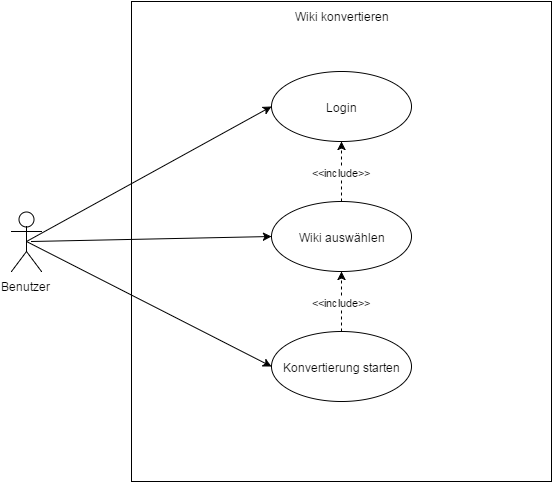
\includegraphics[width=0.85\textwidth]{images/UC_wiki_konvertieren}	
	\caption{Use-Case ''Wiki konvertieren''}
	\end{figure}
	\end{center}
	
	\subsection{Wiki bearbeiten}
	\begin{center}
	\begin{figure}
	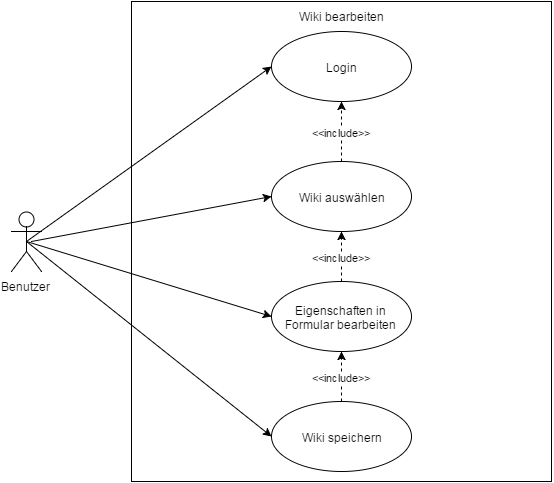
\includegraphics[width=0.85\textwidth]{images/UC_wiki_bearbeiten}	
	\caption{Use-Case ''Wiki bearbeiten''}
	\end{figure}
	\end{center}
		\newpage		
		
\end{appendices}

\end{document}
